Im Folgenden sind die während des Versuchs aufgenommenen Messwerte und die aus diesen 
berechneten Größen tabellarisch dargestellt. An entsprechender Stelle sind Erklärungen
zu den zu den Werten und Rechnungen gegeben.\\

\subsection{Bestimmung der Verdampfungswärme\\ bei Drücken unter einem bar}
\label{sec:gemittelte Verdampfungswärme}
	In \autoref{tab:DataI} sind die, für diese Auswertung verwendeten, Messwerte für Temperatur und 
	Druck dieses Teilversuches zu finden. Dabei sind die angegebenen Messunsicherheiten der Temperaturen
	durch die Einteilung Skala des Thermometers und die Unsicherheiten der Drücke durch die Anzeigegenauigkeit 
	des verwendeten Barometers bestimmt. Letztere änderte sich im Verlauf des Versuchs, beziehungsweise
	musste im Verlauf des Versuchs angepasste werden, da sich die Fluktuation der auf dem Barometer angezeigten
	Messwerte vergrößerte.  
	
		\begin{table}[!h]
			\centering
			\begin{tabular}{|c|c||c|c|}
				\hline
				    Temperatur      &       Druck       &      Temperatur      &       Druck       \\
				$T\,[\si{\kelvin}]$ & $p\,[\si{mbar}] $ & $ T\,[\si{\kelvin}]$ & $ p\,[\si{mbar}]$ \\ \hline\hline
				   %\num{333(1)}     &   \num{244(1)}    & 
				   %\num{335(1)}     &   \num{260(1)}    &    
				   %\num{337(1)}     &   \num{275(1)}    &     
				   %\num{339(1)}     &   \num{291(1)}    &     
				   %\num{341(1)}     &   \num{310(1)}    
				   %\num{343(1)}     &   \num{332(1)}    
				   %\num{345(1)}     &   \num{349(1)}    
				   %\num{347(1)}     &   \num{374(1)}    
				   \num{349(1)}     &   \num{400(1)}    &    \num{361(1)}     &   \num{643(10)}   \\ 
				   \num{351(1)}     &   \num{429(1)}    &    \num{363(1)}     &   \num{694(10)}   \\
				   \num{353(1)}     &   \num{467(1)}    &    \num{365(1)}     &   \num{747(10)}   \\
				   \num{355(1)}     &   \num{506(10)}   &    \num{367(1)}     &   \num{796(10)}   \\
				   \num{357(1)}     &   \num{553(10)}   &    \num{368(1)}     &   \num{821(10)}   \\
				   \num{359(1)}     &   \num{591(10)}   &    \num{369(1)}     &   \num{851(10)}   \\ \hline
			\end{tabular}
			\caption{Werte der Messung bei $p < \SI{1}{bar}$ \label{tab:DataI}}
		\end{table}
	
	Diese Messwerte sind zusammen mit einer Regressionskurve der Form \eqref{eq:pT_exp} in \autoref{fig:pT1}
	aufgetragen, die wegen der halblogarithmischen Skalierung und der Definition $x := \tfrac{1}{T}$ eine Gerade 
	der Form \eqref{eq:pT_ln} darstellt.

	\begin{figure}[!h]
		\centering
		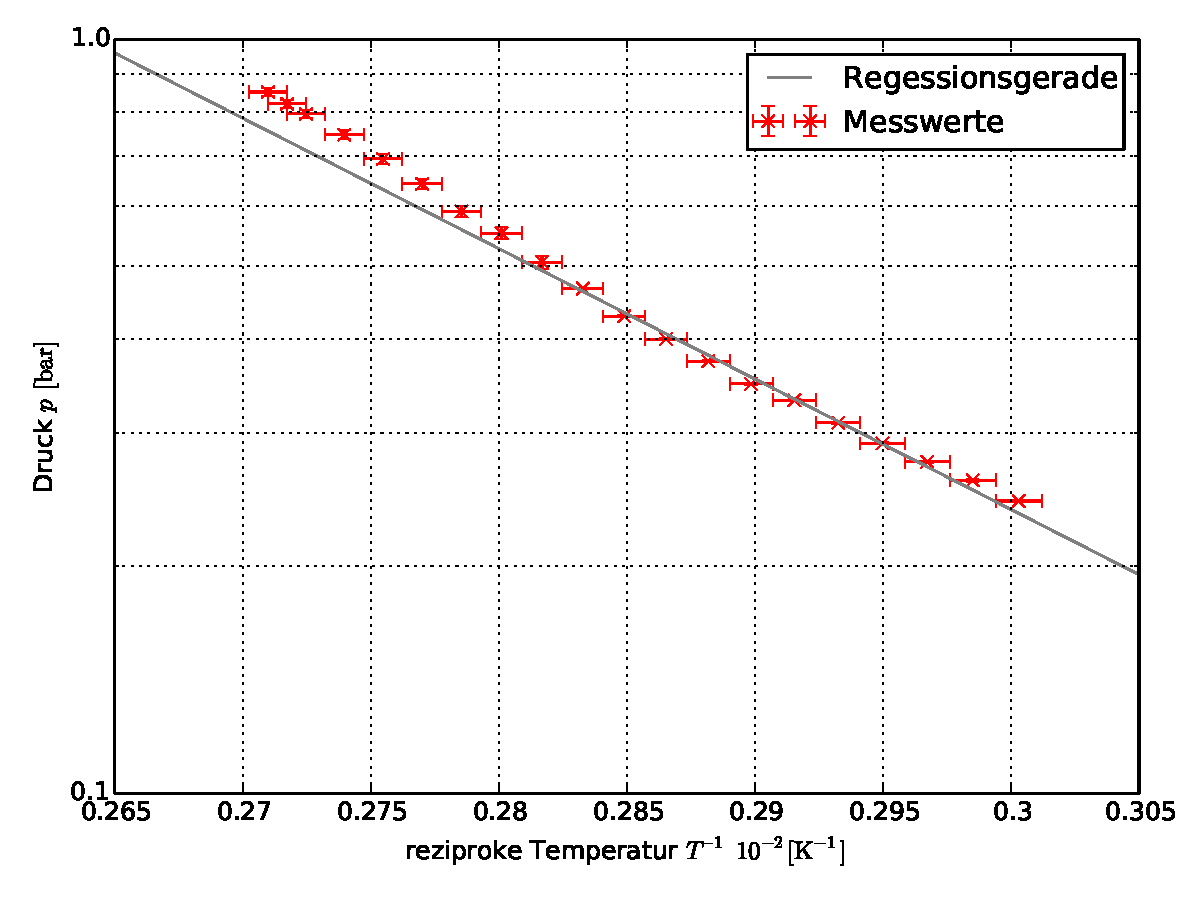
\includegraphics[scale=0.75]{Grafiken/Messreihe_1.pdf}
		\caption{Halblogarithmische Darstellung der Messwerte mit Regressionsfunktion}
		\label{fig:pT1}
	\end{figure}   
	
	Die mit Hilfe der Python Bibliothek \emph{SciPy} \cite{SciPy} bestimmten Parameter der Regerssionsfunktion 
	\begin{empheq}{equation}
		f(x) = Ax + B
	\end{empheq}
	sind:
	\addtocounter{equation}{-1}
	\begin{subequations}
		\begin{empheq}{align}
			\label{eq:A}
			A &= \SI{-0.0491(5)}{\bar\kelvin}\\
			\label{eq:B}
			B &= \SI{13(11)}{\bar}
		\end{empheq}
	\end{subequations} 
	
	 Mit der Steigung  $A = - \tfrac{L}{R}$ und der allgemeinen Gaskonstante $R = \SI{8.314}{\joule\per\mol\per\kelvin}$  \cite{SciPy} lässt
	 sich die Verdampfungswärme aus \eqref{eq:A} zu
	 
	\begin{empheq}{equation*}
	 		\label{eq:L}
	 		L = \SI{4.09(4)e04}{\joule\per\mole}
	\end{empheq}
	berechnen.
	
	\subsection{Bestimmung der inneren Verdampfungswärme}
	\label{sec:innereVerdampfungswärme}
	Für die äußere Verdampfungswärme $L_{a}$ erhält man unter Verwendung der allgemeinen
	Gasgleichung \eqref{eq:allgGas} und der Annahme $V_{F} << V_{D} $ die Näherung
	\begin{empheq}{equation}
	 	\label{eq:L_a}
	 	L_{a} = RT.
	\end{empheq}
	Bei der gegebenen Temperatur $T = \SI{373}{\kelvin}$ ergibt sich damit die notwendige 
	Energie, um das Volumen $V_{F}$ auf $V_{D}$ zu vergrößern zu
	\begin{empheq}{equation*}
		 	L_{a} =  \SI{3101}{\joule\per\mole}\;.
    \end{empheq}  
	Aus der gesamten $L$ und  äußeren Verdampfungswärme $L_{a}$ lässt sich mit \eqref{eq:L_i}
	die innere Verdampfungswärme bestimmen. Durch Skalierung mit der Avogadro-Konstante 
	$N_{A} = \SI{6.022e23}{\per\mole}$ \cite{SciPy} und Umrechnung in $\si{\eV}$\footnote{$\SI{1}{\eV} = \SI{1.602e-19}{\joule}$ \cite{SciPy}},
	erhält man die für die Verdampfung eins einzelnen Wassermoleküls benötigte Energie
	\begin{empheq}{equation*}
			 	L_{i} =  \SI{0.391(4)}{\eV}\;.
	\end{empheq} 
	
	
\subsection{Bestimmung der Temperaturabhängigkeit\\ der Verdampfungswärme}
\label{sec:TAbhängig}
	Die für die folgende Auswertung verwendeten Werte für Druck und Temperatur der zweiten Messung, sind in
	\autoref{tab:DataII} dargestellt. 
	
	\begin{table}[!h]
		\centering
		\begin{tabular}{|c|c||c|c|}
			\hline
			    Temperatur      &      Druck       &     Temperatur      &      Druck       \\
			$T\,[\si{\kelvin}]$ & $p\,[\si{\bar}]$ & $T\,[\si{\kelvin}]$ & $p\,[\si{\bar}]$ \\ \hline\hline
			  \num{343.2(1)}    &  \num{0.90(1)}   &   \num{413.2(1)}    &  \num{2.33(1)}   \\
			  \num{348.2(1)}    &  \num{0.92(1)}   &   \num{418.2(1)}    &  \num{2.72(1)}   \\
			  \num{353.2(1)}    &  \num{0.93(1)}   &   \num{423.2(1)}    &  \num{3.18(1)}   \\
			  \num{358.2(1)}    &  \num{0.95(1)}   &   \num{428.2(1)}    &  \num{3.72(1)}   \\
			  \num{363.2(1)}    &  \num{0.97(1)}   &   \num{433.2(1)}    &  \num{4.36(1)}   \\
			  \num{368.2(1)}    &  \num{1.01(1)}   &   \num{438.2(1)}    &  \num{5.12(1)}   \\
			  \num{373.2(1)}    &  \num{1.05(1)}   &   \num{443.2(1)}    &  \num{5.93(1)}   \\
			  \num{378.2(1)}    &  \num{1.10(1)}   &   \num{448.2(1)}    &  \num{6.84(1)}   \\
			  \num{383.2(1)}    &  \num{1.17(1)}   &   \num{453.2(1)}    &  \num{7.93(1)}   \\
			  \num{388.2(1)}    &  \num{1.26(1)}   &   \num{458.2(1)}    &  \num{9.17(1)}   \\
			  \num{393.2(1)}    &  \num{1.37(1)}   &   \num{463.2(1)}    &  \num{10.54(1)}  \\
			  \num{398.2(1)}    &  \num{1.57(1)}   &   \num{468.2(1)}    &  \num{12.02(1)}  \\
			  \num{403.2(1)}    &  \num{1.74(1)}   &   \num{473.2(1)}    &  \num{13.74(1)}  \\
			  \num{408.2(1)}    &  \num{2.00(1)}   &                     &  \\ \hline
		\end{tabular}
		\caption{Werte der Messung bei $\num{1} \leq p \leq \SI{15}{bar}$ \label{tab:DataII}}
	\end{table}
	Diese Messwerte sind zusammen mit einem Regressionspolynoms 3. Grades der Form
	\begin{empheq}{equation}
		f(x) = Ax^{3} + Bx^{2} + Cx + D
		\label{eq:Reg_Pg3}
	\end{empheq}
	in \autoref{fig:pT2} aufgetragen. Die unter Verwendung von \emph{SciPy} \cite{SciPy} bestimmten Regressionsparameter dieses Polynoms sind:

	\addtocounter{equation}{-1}
	\begin{subequations}
		\begin{empheq}{align}
			 \label{eq:Reg_Pg3a}
			 A &= \SI{0.97(2)}{\bar\per\kelvin\cubed}\\
			 \label{eq:Reg_Pg3b}
			 B &= \SI{-1062(19)}{\bar\per\kelvin\squared}\\
			 \label{eq:Reg_Pg3c}
			 C &= \SI{3.89(8)e05}{\bar\per\kelvin}\\
			 \label{eq:Reg_Pg3d}
			 D &= \SI{-4.7(1)}{\bar}
		\end{empheq}
	\end{subequations}
	
	\begin{figure}[!h]
		\centering
		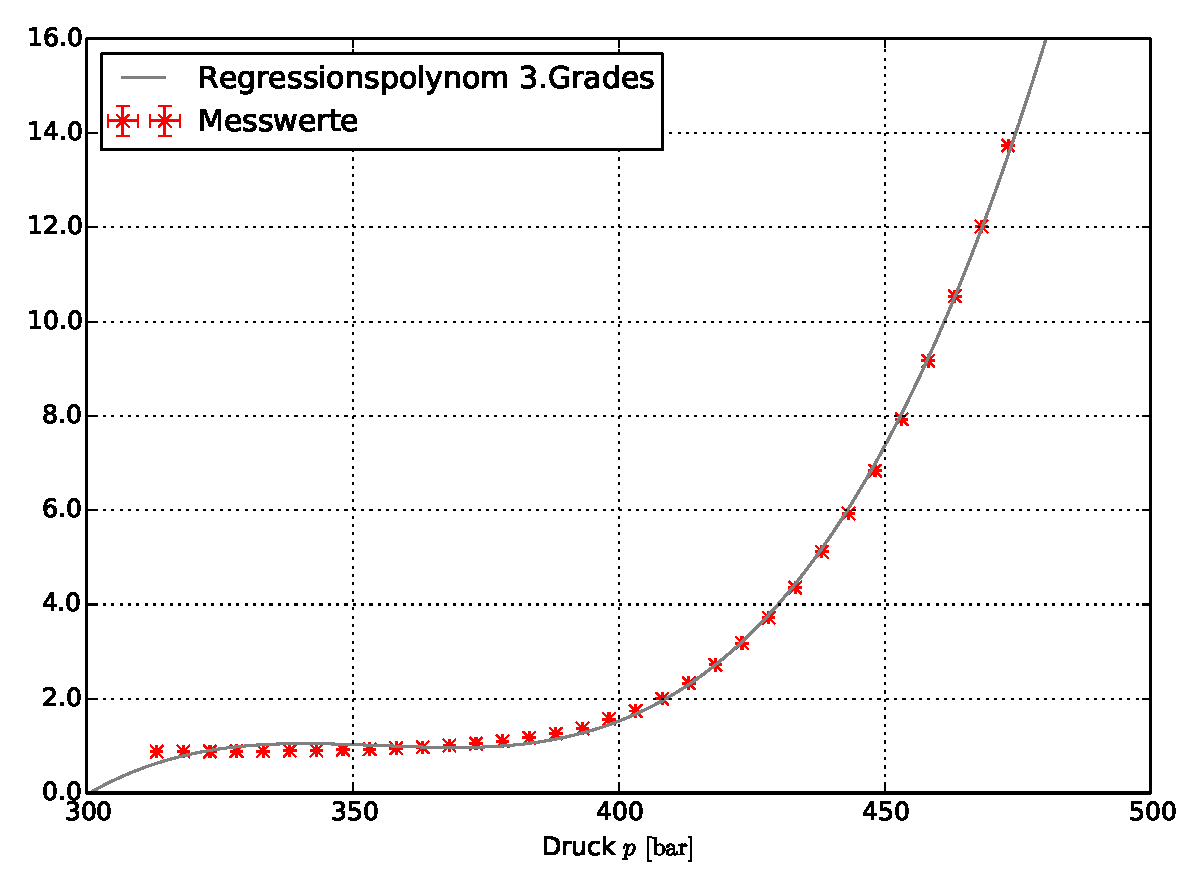
\includegraphics[scale=0.75]{Grafiken/Messreihe_2.pdf}
		\caption{Messwerte und Regressionspolynom der Form $f(x) = Ax^{3} + Bx^{2} + Cx + D$ \label{fig:pT2}}
	\end{figure}
	
	Zur Berechnung der Temperaturabhängigkeit der Verdampungswärme $L$, unter großen Drücken und Temperaturen, wird  
	zunächst \eqref{eq:Clausius} umgestellt, um die Gleichung 
	\begin{empheq}{equation}	
		L = T \cdot (V_{D} - V_{F}) \dod{p}{T}
		\label{eq:L_dpdT}
	\end{empheq}
	zu erhalten.  Der in dieser Gleichung auftretende Differentialquotient kann durch Differentiation des 
	Regressionsploynoms \eqref{eq:Reg_Pg3} mit den Parametern \eqref{eq:Reg_Pg3a} bis \eqref{eq:Reg_Pg3d}  
	zu
	\begin{empheq}{equation}
		 \dod{p}{T} = 3AT^{2} + 2BT + C
		 \label{eq:dpdT}
	\end{empheq} 
	bestimmen werden.
	
	Zur Berechnung des Dampfvolumen $V_{D}$ wird mit \eqref{eq:vanderWaals} eine im Vergleich zur allgemeinen Gasgleichung
	\eqref{eq:allgGas} bessere Näherung verwendet. Durch Auflösen dieser Gleichung nach $V_{D}$ erhält man Mittels \emph{pq-Formel} 
	und mit der Konstanten 
	$ a = \SI{0.9}{\joule\cubic\meter\per\mole\squared}$ \cite{V203} 
	die zwei möglichen Volumina:
	\begin{empheq}{equation}
		V_{D_{1,2}} = \dfrac{RT}{2p} \pm \sqrt{\del{\dfrac{RT}{2p}}^{2} - \dfrac{a}{p}}
		\label{eq:Vd}
	\end{empheq} 
	Die Mittels \eqref{eq:Vd} berechneten Volumina für die Temperaturen und Drücke aus \autoref{tab:DataII} sind in \autoref{tab:Vd}
	aufgelistet. Dabei sind für die Volumina keine Fehler angegeben, da diese für das relevante Volumen $V_{D_{2}}$ von der Größenordnung
	\num{1e-08} sind.
	
	\begin{table}[!h]
		\centering
		\begin{tabular}{|c|c||c|c|}
			\hline
			Volumen \enquote{+} & Volumen \enquote{-} & Volumen \enquote{+} & Volumen \enquote{-}\\
			$V_{D_{1}}\,[\si{d\meter\cubed}]$  & $V_{D_{2}}\,[\si{d\meter\cubed}]$ & $V_{D_{1}}\,[\si{d\meter\cubed}]$  & $V_{D_{2}}\,[\si{d\meter\cubed}]$ \\ \hline\hline
			\num{31.383}  & \num{0.319} & \num{14.476}  & \num{0.267} \\
			\num{31.150}  & \num{0.314} &\num{12.518}  & \num{0.264} \\
			\num{31.263}  & \num{0.310} &\num{10.802}  & \num{0.262} \\
			\num{31.040}  & \num{0.305} &\num{9.310}  & \num{0.260} \\
			\num{30.827}  & \num{0.301} &\num{8.002}  & \num{0.258} \\
			\num{30.010}  & \num{0.297} &\num{6.859}  & \num{0.256} \\
			\num{29.255}  & \num{0.293} &\num{5.959}  & \num{0.255} \\
			\num{28.294}  & \num{0.289} &\num{5.194}  & \num{0.253} \\
			\num{26.943}  & \num{0.286} &\num{4.499}  & \num{0.252} \\
			\num{25.331}  & \num{0.282} &\num{3.903}  & \num{0.252} \\
			\num{23.582}  & \num{0.279} &\num{3.403}  & \num{0.251} \\
			\num{20.810}  & \num{0.276} &\num{2.988}  & \num{0.251} \\
			\num{18.992}  & \num{0.272} &\num{2.612}  & \num{0.251} \\
			\num{16.698}  & \num{0.270} & & \\
			\hline
		\end{tabular}
		\caption{Mögliche Dampfvolumina nach \eqref{eq:Vd} \label{tab:Vd}}
	\end{table}
	
	Daraus ist ersichtlich, dass $V_{D_{1}}$ zwar Lösungen der Gleichung \eqref{eq:Vd} sind, jedoch nicht zu dem Verwendeten Versuchsaufbau
	passen, da der genutzten Stahlbolzen nicht das nötige Volumen hatte um mehrere Liter Wasserdampf zu fassen.\\
	Mit dem Volumen $V_{D} := V_{D_{2}}$,den Temperaturen \autoref{tab:DataII}, den entsprechenden Differntialquotienten \eqref{eq:dpdT} und der Näherung $V_{F} << V_{D}$ erhält man 
	aus \eqref{eq:L_dpdT} die neben den Differntialquotienten in \autoref{tab:L_dpdT} dargestellten Werte für die Verdampfungswärme $L$.
	
	\begin{table}[!h]
		\centering
		\begin{tabular}{|c|c||c|c|}
			\hline
			Differentialquotient & Verdampungswärme & Differentialquotient & Verdampungswärme\\
			$\od{p}{T}\,[\si[prefixes-as-symbols = true]{\milli\bar\per\kelvin}]$ & 
			$L\,[\si{\joule\per\mole}]$ & $\od{p}{T}\,[\si[prefixes-as-symbols = true]{\milli\bar\per\kelvin}]$ & 
			$L\,[\si{\joule\per\mole}]$\\ \hline\hline
				\num{18.8(1)}  & \num{205(1)} & \num{71.0(3)}  & \num{783(3)} \\
				\num{13.1(1)}  & \num{142(1)} & \num{85.6(3)}  & \num{946(4)} \\
				\num{8.78(7)}  & \num{96.0(8)} &\num{101.7(3)}  & \num{1128(4)} \\
				\num{5.97(4)}  & \num{65.3(4)} &\num{119.2(4)}  & \num{1327(4)} \\
				\num{4.61(1)}  & \num{50.4(1)} &\num{138.2(4)}  & \num{1545(5)} \\
				\num{4.71(2)}  & \num{51.4(2)} &\num{158.7(4)}  & \num{1782(5)} \\
				\num{6.25(5)}  & \num{68.4(5)} &\num{180.6(5)}  & \num{2038(6)} \\
				\num{9.26(8)}  & \num{101.2(8)} &\num{203.9(5)}  & \num{2315(6)} \\
				\num{13.7(1)}  & \num{150(1)} &\num{228.8(5)}  & \num{2615(6)} \\
				\num{19.6(1)}  & \num{215(2)} &\num{255.0(5)}  & \num{2938(7)} \\
				\num{27.0(2)}  & \num{296(2)} &\num{282.7(6)}  & \num{3286(7)} \\
				\num{35.8(2)}  & \num{393(2)} &\num{311.9(6)}  & \num{3660(8)} \\
				\num{46.1(2)}  & \num{506(3)} &\num{342.5(6)}  & \num{4064(8)} \\
				\num{57.8(3)}  & \num{636(3)} & & \\
			\hline
		\end{tabular}
		\caption{Differntialquotient und Temperaturabhängige Verdampungswärme \label{tab:L_dpdT}}
	\end{table}
	
	In \autoref{fig:L_T} sind die berechneten Verdampfungswärmen aus \autoref{tab:L_dpdT} zusammen mit 
	einem Regressionspolynom 2. Grades der Form 
	\begin{empheq}{equation}
		f(x) = Ax^{2} + Bx + C
	\end{empheq} 
	gegen die Temperaturen aus \autoref{tab:DataII} aufgetragen.
	Die mit SciPy bestimmten Regressionsparamter für dieses Polynom sind:
	\addtocounter{equation}{-1}
	\begin{subequations}
		\begin{empheq}{align}
				A &= \SI{0.334(2)}{\joule\per\mole\per\kelvin\squared}\\
				B &= \SI{-244(2)}{\joule\per\mole\per\kelvin}\\
				C &= \SI{4.47(4)e04}{\joule\per\mole}
		\end{empheq}
	\end{subequations} 
	
	\begin{figure}[!h]
		\centering
		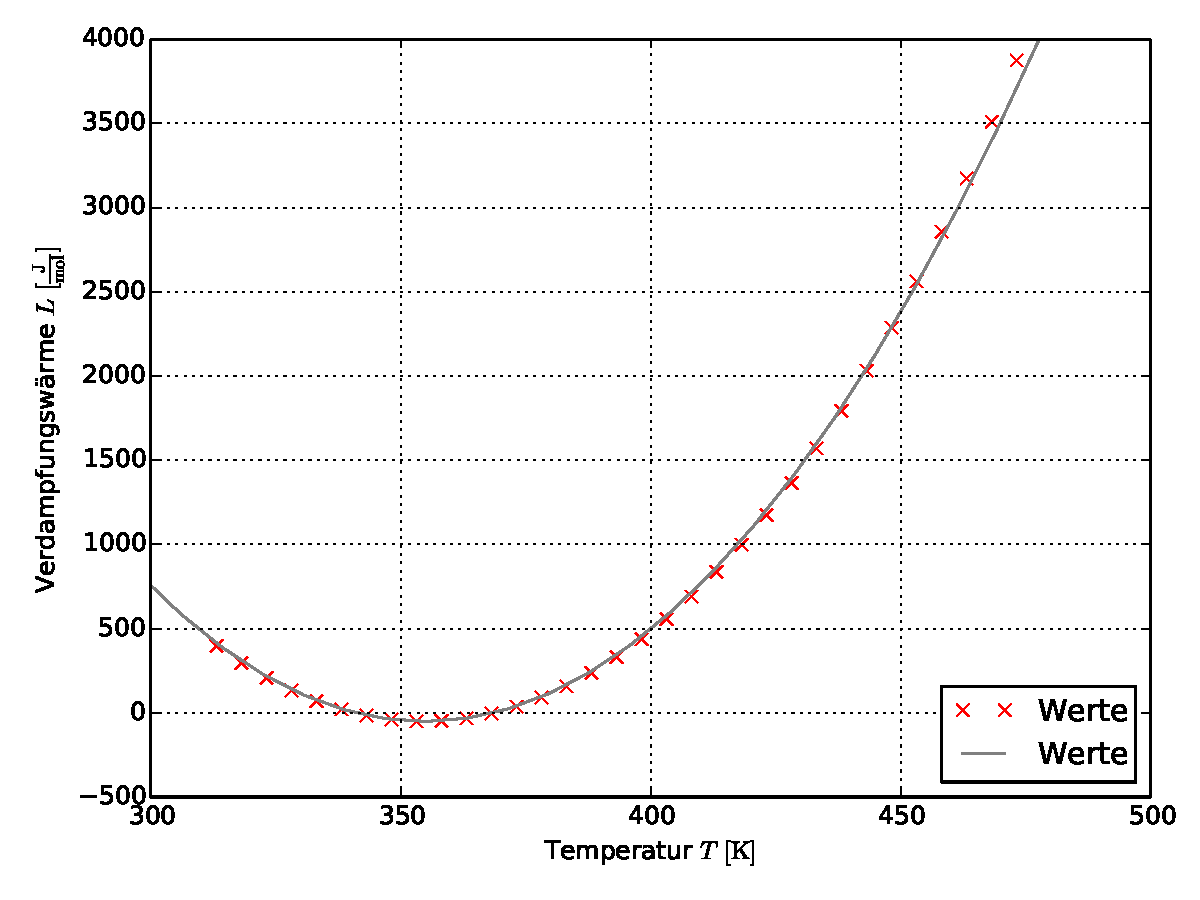
\includegraphics[scale=0.75]{Grafiken/Verlauf_LT.pdf}
		\label{fig:L_T}
	\end{figure}
\newpage